

\documentclass[11pt,a4paper]{scrreprt}
\usepackage[utf8]{inputenc}
\usepackage[ngerman]{babel}
\usepackage[T1]{fontenc}
\usepackage{relsize} 	
\usepackage{helvet}
\usepackage{hyperref}
\usepackage{amsmath}
\usepackage{amsfonts}
\usepackage{amssymb}
\usepackage[a4paper, left=2cm, right=2cm, top=2cm, bottom=2cm]{geometry}
\usepackage{titlesec}
\titleformat{\chapter}
   {\normalfont\large\bfseries}{\thechapter\quad}{0cm}{}\titlespacing{\chapter}{0pt}{0pt}{6pt}
\titleformat{\section}
   {\normalfont\large\bfseries}{\thesection\quad}{0cm}{}
\titlespacing{\section}{0pt}{12pt}{6pt}
\titleformat{\subsection}
   {\normalfont\large\bfseries}{\thesubsection\quad}{0cm}{}
\titlespacing{\subsection}{0pt}{12pt}{6pt}
\setlength{\parindent}{0em}
%\usepackage{ragged2e}
\usepackage{graphicx}
\usepackage{setspace}
\onehalfspacing
\newcommand{\abbildung}[1]{\figurename\ \ref{#1}}
\usepackage{tabularx}
\usepackage{enumitem}






\begin{document}


\begin{titlepage}


\begin{center}
	
	
\includegraphics[height=6cm]{LogoIU}
	
	\vspace{4cm}
	
	\LARGE{\textbf{Hausarbeit}}
	\vspace{2cm}
	
	\LARGE{\textbf{DLMDWPMP01 - Programmieren mit Python}}
\end{center}
\vspace{5cm}

\begin{flushleft}
\begin{tabular}{lcl}

Erstellt von: & & Steffen Baumann \\ 

Matrikelnummer: && IU14089925 \\ 

Studiengang: & & Informatik (Master of Science) \\ 

Tutor: & & Dr. Thomas Kopsch \\

\\



vorgelegt am: &  & 16.04.2024 \\ 

\end{tabular} 
\end{flushleft}
\end{titlepage}


\clearpage


\tableofcontents
\thispagestyle{empty}
\clearpage







\pagenumbering{arabic} 


\chapter{Einleitung}
\label{cha:Einleitung}
Die Programmiersprache Python ist eine einfach zu erlernende Sprache, die es dem Anwender erlaubt, komplexe Programme für verschiedene Anwendungsgebiete zu entwickeln (Theis, 2017, S.17).
Die Grundlage dieser Hausarbeit bilden drei CSV-Dateien, die vier Trainingsfunktionen („train.csv“), 50 Idealfunktionen („ideal.csv“) sowie 100 Testpunkte („test.csv“) beinhalten.
Ziel dieser Hausarbeit ist es, ein Python Programm zu entwickeln, das die drei CSV-Dateien importiert, den Inhalt verarbeitet und abschließend die Daten in eine SQLite-Datenbank speichert.\\
Die folgenden zwei Kapitel geben die Aufgabenstellung, unterteilt in zwei Aufgabenteile, wieder. Im Hauptteil werden die verwendeten Bibliotheken vorgestellt sowie die Struktur des Programms erklärt. Im Schlussteil wird ein Resümee gezogen, wobei auch darauf eingegangen wird, welche Vor- sowie Nachteile das erzeugte Python Programm besitzt. 


\section{Aufgabenteil 1}
\label{sec:Aufgabenteil1}

In einem ersten Abschnitt soll zu den vier Trainingsfunktionen jeweils eine bestmögliche Idealfunkti-on ermittelt werden. Eine Idealfunktion ist dann die bestmögliche Passung, wenn die Summe aller quadratischen y-Abweichungen minimal ist. Dieses Kriterium kann mit folgender Formel (Least-Square) berechnet werden:
\begin{equation}
\label{eq:leastsquare}
y_{A}= \frac{1}{N}\sum_{i}^{N} (y_{i}-\bar{y_{i}})^2 
\end{equation}
\begin{flushleft}
$y_{i}$ = Y-Wert der Trainingsfunktion \\
$\bar{y_{i}}$ = Y-Wert der Idealfunktion
\end{flushleft}
Sind die besten Passungen aus Trainings- und Idealfunktion bestimmt, sollen die jeweiligen Ergebnisse logisch visualisiert werden.

\section{Aufgabenteil 2}
\label{sec:Aufgabenteil2}
Die vier bestmöglichen Idealfunktionen aus Aufgabenteil 1 werden nun zur Analyse der 100 Testpunkte verwendet. Es wird geprüft, ob die Testpunkte einer oder mehreren Idealfunktionen zugeordnet werden können. Um zu entscheiden, ob ein Testpunkt zu einer Idealfunktion passt, wird zuerst die Abweichung zwischen dem Y-Wert des Testpunktes und dem Y-Wert der Idealfunktion berechnet. Ist die Abweichung kleiner als das Testkriterium (maximale Y-Abweichung zwischen Ideal – und Trainingsfunktion, multipliziert mit $\sqrt{2}$), gilt der Testpunkt als anpassbar. Auch die Ergebnisse aus Aufgabenteil 2 sollen logisch visualisiert werden. 

\chapter{Python-Bibliotheken und -Module}
Dieses Kapitel beschreibt die in dieser Hausarbeit verwendeten Python-Bibliotheken sowie -Module und erläutert, welche Abläufe im Programm sie vereinfachen.
\section{Pandas-Bibliothek}
\label{sec:Pandas}
Die Pandas-Bibliothek ist spezialisiert für das umfangreiche Arbeiten mit strukturierten oder tabellarischen Daten. Sie eignet sich besonders gut für die Manipulation, Vorbereitung und Bereinigung von Daten (McKinney, 2023, S.23).\\
Für die Bearbeitung der Aufgabe wird das Pandas-Dataframe inklusive der anwendbaren Funktionen verwendet. Ein Pandas-Dataframe ist eine tabellenartige, geordnete Datenstruktur, wobei jede Zeile sowie Spalte einen Index besitzt (McKinney, 2023, S.148).\\
In dieser Hausarbeit wird die Pandas-Bibliothek verwendet, um die Daten aus den CSV-Dateien zu importieren und zu speichern. Mit Hilfe der zur Pandas-Bibliothek gehörenden Methoden werden die erzeugten Pandas-Dataframes bearbeitet und so manipuliert, dass sie die Weiterverarbeitung zum Erreichen des Ziels der Aufgabenstellung ermöglichen. 
\section{Matplotlib-Bibliothek}
Matplotlib ist eine der populärsten Bibliotheken zur Visualisierung von Daten in Python. Sie ermöglicht es dem Anwender, verschiedene Arten von Diagrammen und Grafiken zu erstellen. Hierzu zählen unter anderem Scatterplots, Liniendiagramme und Balkendiagramme (Matthes, 2019, S.306). Die Matplotlib-Bibliothek besitzt die Fähigkeit, mit einer Vielzahl von Betriebssystemen und grafischen Ausgabegeräten zu interagieren (VanderPlas, 2018, S.245).\\
Alle in dieser Hausarbeit erstellten Grafiken zur Visualisierung der Ergebnisse werden auf Basis der Matplotlib-Bibliothek erstellt. Für Aufgabenteil 1 werden ausschließlich Liniendiagramme erstellt. Die Ergebnisse aus Aufgabenteil 2 werden in einer Grafik visualisiert, die eine Liniendiagramm und einen Scatterplot kombiniert. \\
Für eine bessere Lesbarkeit der Diagramme/Grafiken werden Titel, Legende und Achsenbeschriftung hinzugefügt (Matthes, 2019, S.308).

\section{SQL-Alchemy-Bibliothek}
\label{sec:SQL}
Die SQL-Alchemy-Bibliothek dient als Verbindungselement zwischen dem Python-Code und einer Datenbank. SQL-Alchemy konvertiert Python-Funktionsaufrufe in die entsprechenden SQL-Anweisungen. Es werden mehrere Datenbanken, bspw. MySQL oder SQLite, unterstützt (Campesato, 2023, S.253).\\
In dieser Hausarbeit sollen die Ergebnisse in einer SQLite-Datenbank gespeichert werden. SQLite ist eine prozessinterne Bibliothek, die eine in sich geschlossene, serverlose, konfigurationsfreie SQL-Datenbank-Engine beinhaltet. Der Code für SQLite ist öffentlich zugänglich, wobei die SQLite-Datenbank die am weitesten verbreitete Datenbank ist (Campesato, 2023, S.260+261).\\
Mit Hilfe der SQL-Alchemy-Bibliothek wird im Python-Programm die Verbindung zur SQLite-Datenbank hergestellt, eine Tabelle angelegt und die Daten in die Datenbank überschrieben. Das Ergebnis ist abschließend jeweils eine lokale SQLite-Datei für den Trainings-, Ideal- und Testdatensatz.

\section{UnitTest-Bibliothek}
\label{sec:UnitTest}
Das Testen des Python-Programms ist ein wichtiger Schritt bei der Entwicklung eines Python-Codes. Es wird sichergestellt, dass die Funktionalität des Programms wie erwartet gegeben ist. Fehler können aufgedeckt und frühzeitig behoben werden. Eine Möglichkeit, das Python-Programm wie beschrieben zu testen, bietet die UnitTest-Bibliothek. Sie ist einer der beliebtesten Test-Bibliotheken und gehört zu den Standardbibliotheken von Python (Kapil, 2019, S.238-240). \\
Mit der UnitTest-Bibliothek wird im vorliegenden Python-Programm die Funktionalität der Module der einzelnen Klassen überprüft. Es wird geprüft, ob Berechnung korrekt durchgeführt werden und ob Argumente der Klassen richtig zurückgegeben werden. Außerdem wird das Anlegen von Instanzen der erzeugten Klassen überprüft.  


\section{Tkinter-Modul}
Das Tkinter-Modul ist eine Schnittstelle zur Tk-Bibliothek, die zu den Standardbibliotheken von Python gehört. Durch das Tkinter-Modul ist es möglich, grafische Oberflächen für kleinere Anwendungen zu erstellen (Theis, 2017, S.371). \\
In dem Python-Programm wird das Modul filedialog des Pakets Tkinter verwendet, das vorgefertigte Dateidialoge bereitstellt. Die Dateidialoge fordern den Nutzer des Python-Programms dazu auf, Dateien oder Ordner auszuwählen, um diese im Python-Programm hineinzuladen (Ernesti, 2020, S.869).\\
Das Modul filedialog kommt in dieser Hausarbeit jedoch nur dann zum Einsatz, wenn die als Default eingebetteten Dateipfade nicht existieren. Um einen Abbruch des Programms zu verhindern, müssen schließlich die drei CSV-Dateien manuell ausgewählt werden. 


\section{OS-Modul}
Das os-Modul ermöglicht es, betriebssystemabhängige Funktionalitäten zu nutzen (OS-DOKU).\\ Im erstellten Python-Programm werden mit Hilfe des os-Moduls die Datei-Pfade der zu importierenden CSV-Dateien überprüft. Existieren die als Default implementierten Dateipfade nicht, wird der Benutzer aufgefordert, die drei CSV-Dateien manuell auszuwählen. 

\section{Math-Modul}
Durch das math-Modul erlangt der Anwender Zugang zu mathematischen Funktionen. Hierzu zählen unter anderem die trigonometrischen Funktionen (Theis, 2017, S.89-91). Für die Berechnung des Testkriteriums in Aufgabenteil 2 wird die Berechnung der Quadratwurzel benötigt, die ebenfalls eine Funktion des math-Moduls ist. 
\chapter{Struktur des Python-Programms}

Dieses Kapitel behandelt die Struktur des entwickelten Python-Programms. Die Aufgabenstellung gibt vor, dass eine objektorientierte Programmierung angewendet werden soll. Außerdem sollen sowohl Standard- als auch user-definierte Exception-Handlings sinnvoll verwendet werden und Unit-Tests, wo immer es sich anbietet, implementiert werden (siehe Kapitel \ref{sec:UnitTest}). In den folgenden Unterkapiteln werden die genannten Anforderungen vertieft und die Umsetzung im Python-Code erläutert. 


\section{Objektorientierte Programmierung}
\label{sec:OOP}
Unter einer objektorientierten Programmierung ist zu verstehen, dass alle Elemente, mit denen ein Python-Programm erstellt wird, eine Instanz einer Klasse ist. Dies betrifft einzelne Zahlen genauso wie Listen, Dictionaries usw. (Ernesti, 2020, S.381). \\
Grundlage der objektorientierten Programmierung sind sogenannte Klassen, die mit Eigenschaften (Attribute) und Methoden (Funktionen) ausgestattet werden. Es können nun im Programm-Code mehrere Objekte (Instanzen) dieser Klassen erzeugt werden und die entsprechenden Methoden auf die Objekte angewendet werden. Weiterhin besteht die Möglichkeit, dass einzelne Klassen von einer anderen Klasse erben. Es wird eine Basisklasse (Eltern-Klasse) definiert, die ihre Eigenschaften und Methoden an die abgeleitete Klasse (Kind-Klasse) vererbt. Ähnliche Objekte mit identischen Eigenschaften und Methoden können so vereinfacht erzeugt werden (Theis, 2017, S.203).\\
Python ermöglicht es dem Anwender, bei der Definition der Attribute und Methoden einer Klasse aus drei Sichtbarkeitstufen zu wählen. Auf Attribute und Methoden, die als public deklariert werden, kann von außerhalb der Klasse ohne Einschränkungen zugegriffen werden. Ähnlich verhält es sich bei der Sichtbarkeitsstufe protected, die häufig in Vererbungshierachien Anwendung findet. Prinzipiell ist der Zugriff auf die Attribute und Methoden von außen uneingeschränkt möglich. Per Konvention wird jedoch festgelegt, dass die Sichtbarkeitsstufe protected behandelt wird wie die Sichtbarkeitsstufe privat. Hierbei ist kein Zugriff auf Attribute und Methoden von außen möglich (Steyer, 2018, S.161).\\
In dieser Hausarbeit werden zur Bearbeitung der Aufgabenstellung drei Basisklassen erzeugt, wobei eine Basisklasse drei abgeleitete Klassen besitzt. Zusätzlich sind in dem Python-Programm vier Klassen zum Abfangen von Fehlern (Exception-Handling) implementiert. Im Folgenden werden die drei zur Lösung der Aufgabenstellung verwendeten Klassen sowie ihre Funktionalitäten erläutert. 
Die erstellten Klassen des Python-Programms besitzen Attribute der Sichtbarkeitsstufe privat oder protected. Um auf diese Attribute zugreifen zu können, gibt es für jedes Attribut eine Getter- und Setter-Methode (Steyer, 2018, S.162+163). Diese Methoden beginnen im Python-Code jeweils mit hole (get) und setze (set). Um die folgenden Grafiken nicht zu überladen, werden sie nicht aufgeführt.  

\subsection{Klasse Datensatz}
\label{sub:Datensatz}
Die Klasse Datensatz bildet die Grundlage für die Verarbeitung der Daten aus den CSV-Dateien. Sie ist zudem eine Elternklasse der Klasse Funktion, die in Kapitel \ref{sub:Funktion} erläutert wird. \abbildung{fig:Datensatz} zeigt die Attribute und Methoden der Klasse Datensatz sowie die entsprechenden Kindklassen. 
\begin{figure}[!h]
	\centering
	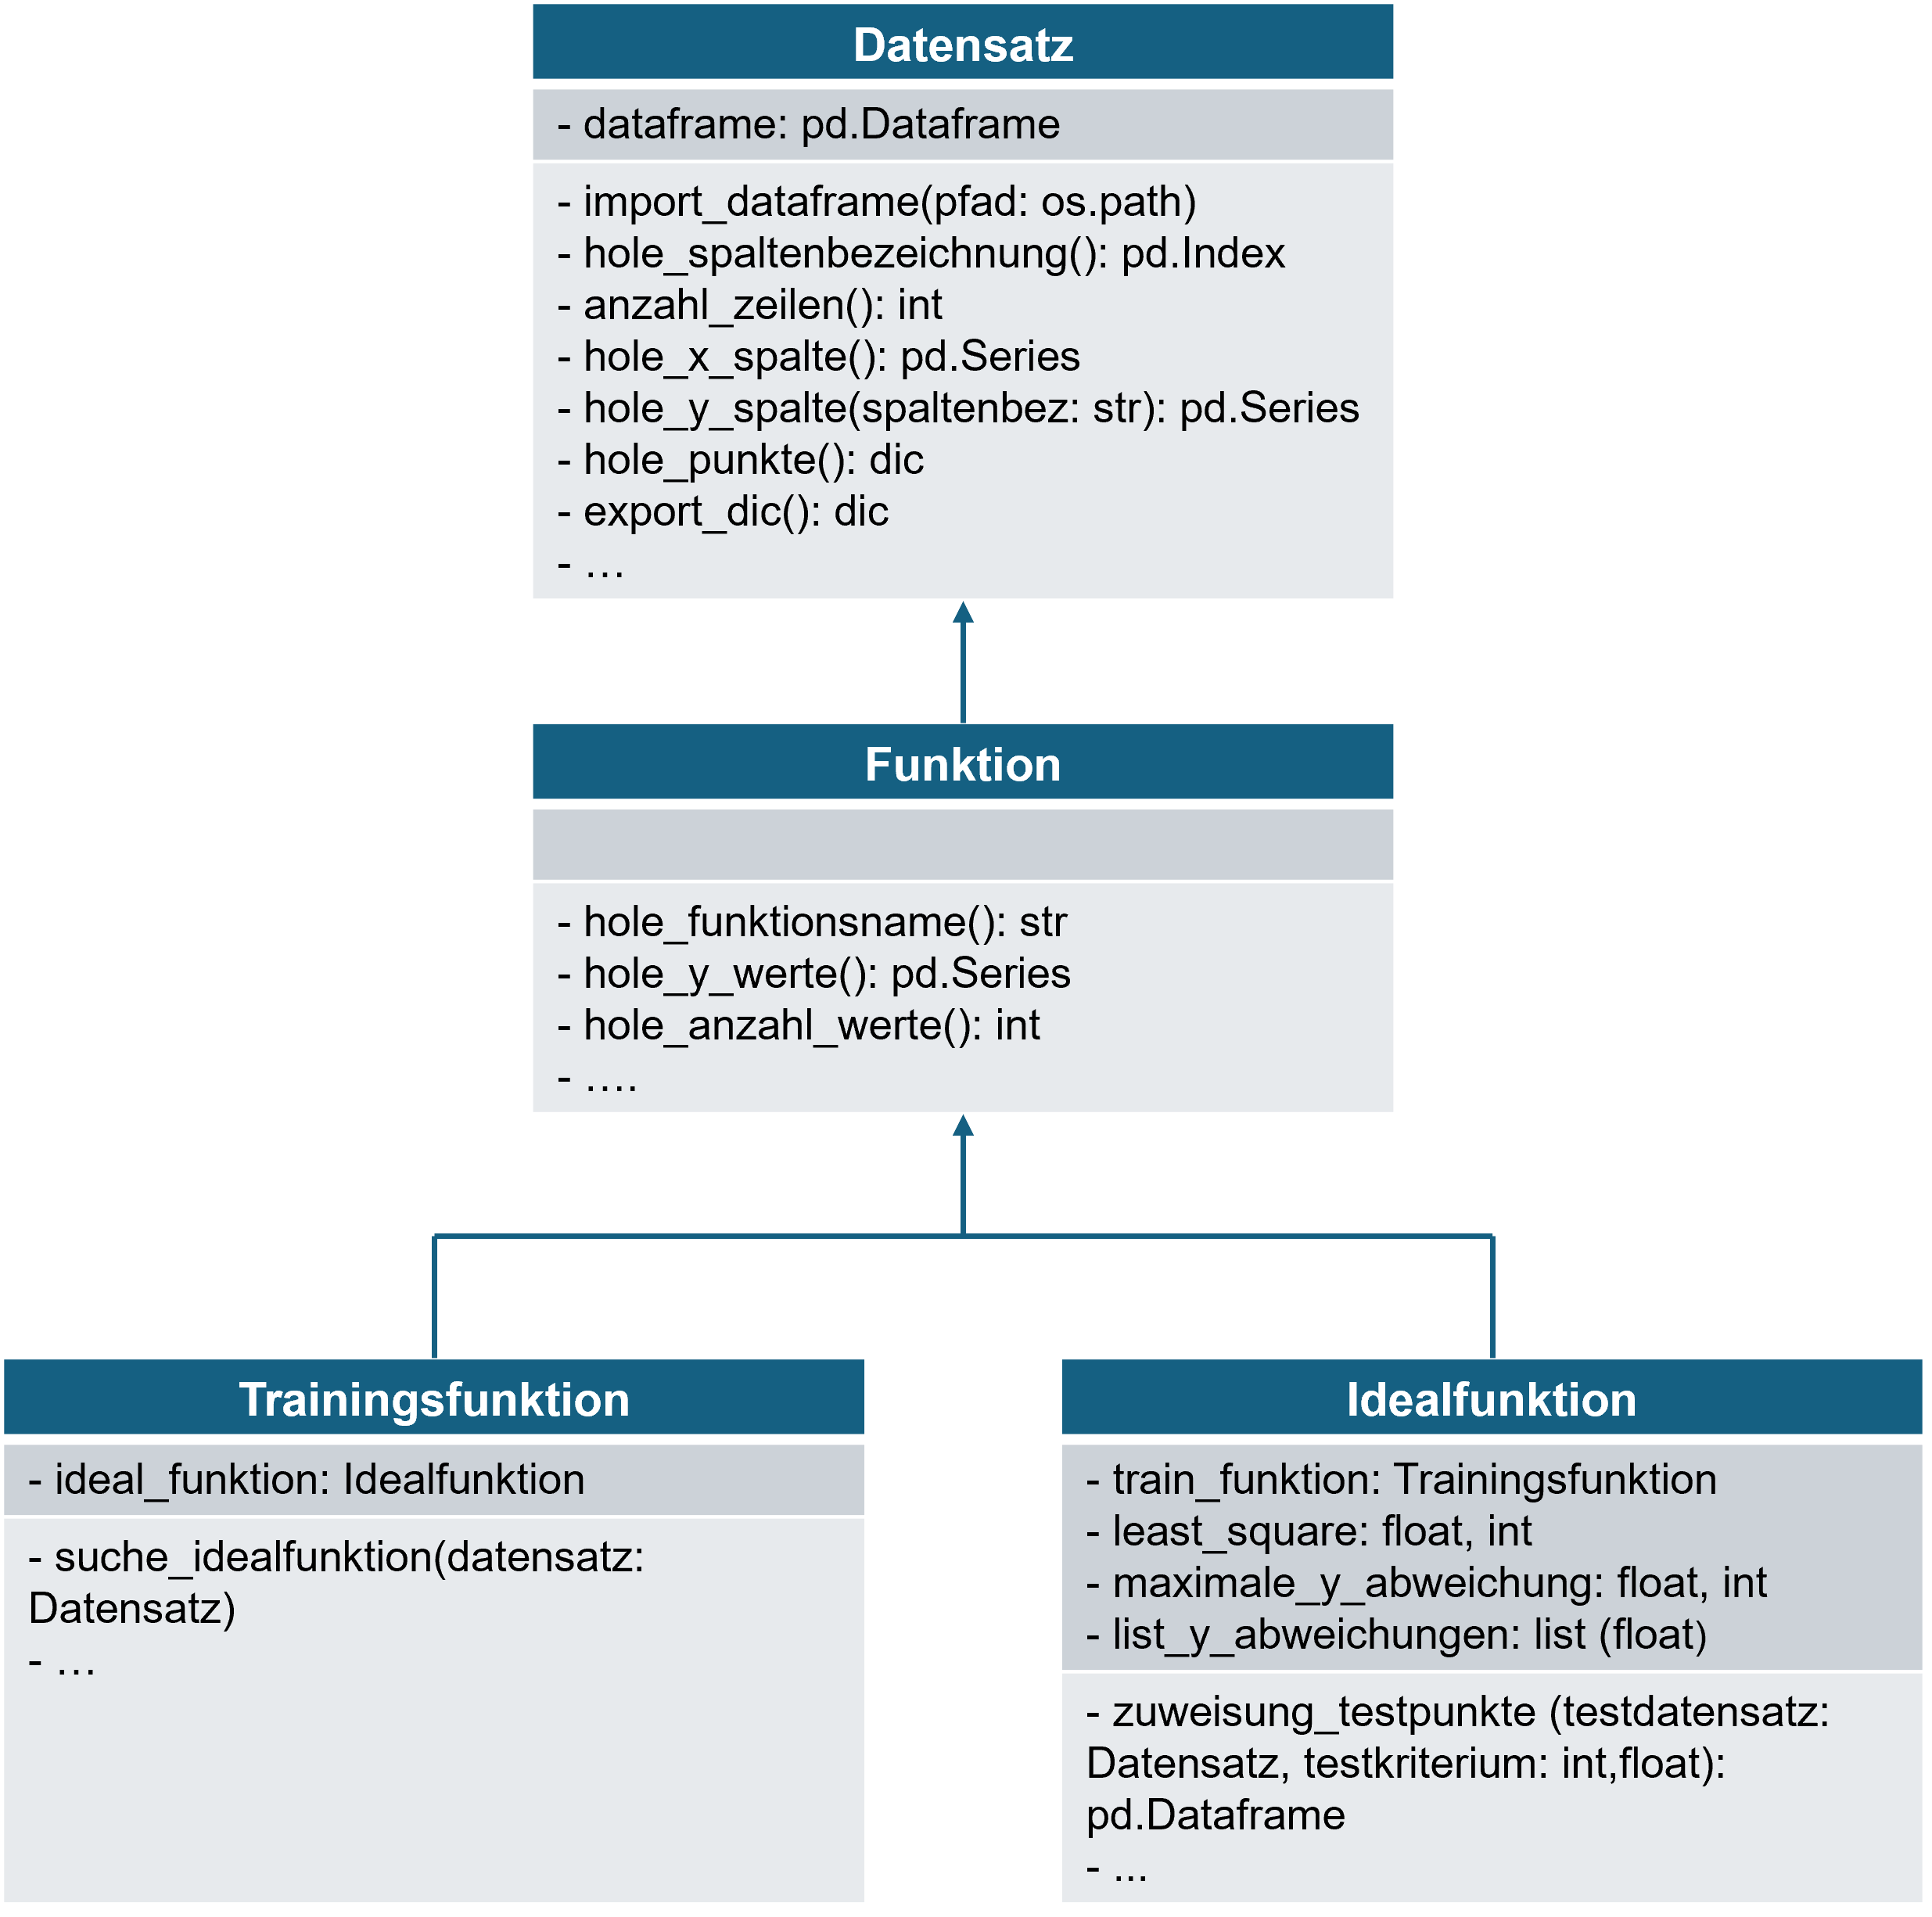
\includegraphics[scale=0.78]{Grafik_Klasse_Datensatz_Funktion}
	\caption{Attribute und Methoden der Klasse Datensatz}
	\label{fig:Datensatz}
\end{figure}

Die Grafik zeigt, dass die Klasse Datensatz nur ein Attribut besitzt (dataframe). Bei der Erstellung der Klasse muss jedoch nicht zwingend eine Variable für das Attribut übergeben werden. In diesem Fall bekommt das Attribut dataframe den Wert einer leeren Zeichenkette. Somit kann eine Instanz der Klasse Datensatz entweder mit einer leeren Zeichenkette oder einem Pandas-Dataframe (siehe Kapitel \ref{sec:Pandas}) erzeugt werden. \\
Wird einer Instanz der Klasse Datensatz bei der Erzeugung kein Pandas-Dataframe zugewiesen, bietet die Methode import\_dataframe() die Möglichkeit, das Attribut dataframe durch den Import einer CSV-Datei zu belegen. Hierbei wird aus den Daten der CSV-Datei ein Pandas-Dataframe erzeugt und gespeichert.\\
Die in der folgenden Tabelle \ref{tab:Klasse_Datensatz} beschriebenen Methoden können jeweils nur ausgeführt werden, wenn dem Attribut dataframe ein Pandas-Dataframe zugewiesen ist. Daher wird vor jeder Ausführung der Methoden unter Verwendung eines Exception-Handlings überprüft, ob es sich um ein Pandas-Dataframe oder eine leere Zeichenkette handelt. 
\begin{table}[!h]
\centering
\begin{tabularx}{0.95\textwidth}{|l|X|}
\hline
\textbf{Methode} & \textbf{Funktionalität}\\
\hline
hole\_spaltenbezeichnung() & Die Spaltenbezeichnungen des Pandas-Dataframes werden ausgegeben (z.B. x,y1,…).\\
\hline
anzahl\_zeilen() & Die Anzahl der Zeilen des Pandas-Dataframes wird zurückgegeben. Die Anzahl der Zeilen ist äquivalent zu der Anzahl der X- und Y-Werte der Funktionen.\\
\hline
hole\_x\_spalte() & Die X-Werte der Funktionen werden zurückgegeben.\\
\hline
hole\_y\_spalte(spaltenbez) & Die Y-Werte einer bestimmten Spalte (Funktion) werden zurückgegeben.\\
\hline
hole\_punkte() & Die Punkte (X,Y)  der einzelnen Funktionen werden zurückgegeben. \\
\hline
export\_dic() & Das Pandas-Dataframe wird als Dictionary zurückgegeben.\\
\hline
\end{tabularx}
\caption{Methoden der Klasse Datensatz}
\label{tab:Klasse_Datensatz}
\end{table}

Bei dem Großteil der in Tabelle \ref{tab:Klasse_Datensatz} beschriebenen Methoden der Klasse Datensatz wird lediglich auf Funktionen des Datentyps Pandas-Dataframe zurückgegriffen. Die Klasse Datensatz dient nicht dazu, Berechnungen oder Ähnliches durchzuführen. Sie soll das Arbeiten mit einem Pandas-Dataframe erleichtern und anwenderfreundlicher gestalten. Die Bezeichnungen der Methoden sind auf die zu verarbeitenden Daten dieser Hausarbeit abgestimmt. Somit kann es bei der Anwendung der Klasse Datensatz auf abweichende Datenstrukturen zu Verständnisproblemen kommen. Es ist z.B. zwingend notwendig, dass das Pandas-Dataframe in der ersten Spalte die X-Werte der Funktionen beinhaltet, um bei der Anwendung der Methode hole\_x\_spalte() ein korrekten Rückgabewert zu erhalten.\\
Zum einen wird die Klasse Datensatz verwendet, um die Daten aus den gegebenen CSV-Dateien zu importieren. Durch die implementierten Methoden werden die Daten gespeichert und für weitere Berechnungen aufbereitet. \\
Zum anderen werden die Funktionalitäten des Pandas-Dataframes, und damit auch der Klasse Datensatz, genutzt, um die Daten mit geringem Aufwand in eine SQLite-Datenbank zu exportieren. 

\subsection{Kindklasse Funktion}
\label{sub:Funktion}
Die Klasse Funktion ist eine Kindklasse der Klasse Datensatz. Sie besitzt wiederum mit den Klassen Trainings- und Idealfunktion zwei abgeleitete Klassen(siehe \abbildung{fig:Datensatz}). Mit Hilfe dieser Klassen werden die zur Lösung der Aufgabenstellung benötigten Berechnungen durchgeführt. \\
Die Klasse Funktion besitzt, neben dem Attribut dataframe aus der Elternklasse, kein weiteres Attribut. Jedoch ist es bei der Erstellung einer Instanz der Klasse Funktion zwingend erforderlich, ein Pandas-Dataframe zu übergeben. Wird kein Pandas-Dataframe übergeben, wird das Programm mit Hilfe des Exception-Handlings abgebrochen. Die Klasse Funktion verarbeitet nur die ersten beiden Spalten des Pandas-Dataframes, da hier per Definition die X- sowie Y-Werte der Funktion zu finden sind. Tabelle \ref{tab:Klasse_Funktion} zeigt die zur Klasse Funktion gehörenden Methoden und beschreibt ihre Funktionalität. 

\begin{table}[!h]
\centering
\begin{tabularx}{0.95\textwidth}{|l|X|}
\hline
\textbf{Methode} & \textbf{Funktionalität}\\
\hline
hole\_funktionsname() & Der Funktionsname des Pandas-Dataframes (Index der zweiten Spalte) wird zurückgegeben (z.B. y1).\\
\hline
hole\_y\_werte() & Die Y-Werte der Funktion (zweite Spalte) werden zurückgegeben.\\
\hline
\end{tabularx}
\caption{Methoden der Klasse Funktion}
\label{tab:Klasse_Funktion}
\end{table}

Da bei der Erzeugung einer Instanz der Klasse Funktion die Konstruktor-Methode der Elternklasse Datensatz aufgerufen wird, ist die Grundlage der Klasse Funktion ebenfalls ein Pandas-Dataframe (siehe \abbildung{fig:Datensatz}). Somit kann mit der Klasse Funktion  problemlos auf die Methoden der Elternklasse Datensatz zugegriffen werden. Die Funktionalität aller in Tabelle \ref{tab:Klasse_Funktion} gezeigten Methoden basiert auf Funktionen eines Pandas-Dataframes. Auch in diesem Fall stellen die Bezeichnungen der Methoden der Klasse Funktion eine Beziehung zu der Datenstruktur der vorgegebenen CSV-Dateien her. \vspace{6pt}\\ 
\vspace{6pt}\textbf{Klasse Trainingsfunktion}\\
Die Klasse Trainingsfunktion beinhaltet mit der Methode suche\_idealfunktion(datensatz) die eigentliche Funktion zur Bearbeitung von Aufgabenteil 1 (siehe Kapitel \ref{sec:Aufgabenteil1}). Einer Trainingsfunktion wird bei der Anwendung dieser Methode ein Datensatz, also ein Pandas-Dataframe, zur weiteren Verarbeitung zugewiesen. Im Regelfall ist dies der Datensatz der Idealfunktionen. Es wird über alle Funktionen des Pandas-Dataframes der Idealfunktionen iteriert. Pro Spalte wird eine Vergleichsfunktion angelegt, die eine Instanz der Elternklasse Funktion ist. Sie dient lediglich als Vergleichsobjekt. Hierzu werden Methoden der Klasse Funktion, bspw. hole\_y\_werte(), benötigt. Nun wird über die Y-Werte der Vergleichsfunktion iteriert und jeweils die Y-Abweichung zum entsprechenden Y-Wert der Trainingsfunktion berechnet. Die Y-Abweichungen werden quadriert und summiert, um den Least-Square-Wert zu berechnen (siehe Formel \ref{eq:leastsquare}). Die Vergleichsfunktion mit dem geringsten Least-Square-Wert wird schließlich als Instanz der Klasse Idealfunktion unter dem Attribut ideal\_funktion gespeichert. Zusätzlich wird zur Anwendung des Testkriteriums für Aufgabenteil 2 (siehe Kapitel \ref{sec:Aufgabenteil2}) die maximale Abweichung zwischen einem Y-Wert der Trainingsfunktion und dem entsprechenden Y-Wert der Idealfunktion bestimmt.\vspace{6pt}\\ 
%
\vspace{6pt}\textbf{Klasse Idealfunktion}\\
Instanzen der Klasse Idealfunktion dienen zum einen als Speicherort der bestimmten Funktionen zur entsprechenden Trainingsfunktion. Die Klasse Idealfunktion beinhaltet neben dem Attribut der Elternklasse (dataframe) vier weitere Attribute. Bei der Erzeugung einer Instanz der Klasse Idealfunktion müssen neben einem Pandas-Dataframe der Idealfunktion zusätzlich folgende Attribute zugewiesen werden (siehe \abbildung{fig:Datensatz}):
\setlist{noitemsep}
\begin{itemize}
\item Least-Square-Wert
\item maximale Y-Abweichung
\item Liste alle Y-Abweichungen zur Trainingsfunktion
\item Trainingsfunktion  
\end{itemize}
Zum anderen wird mit Hilfe der Methode zuweisung\_testpunkte() die Berechnung für Aufgabenteil 2 (siehe Kapitel \ref{sec:Aufgabenteil2}) durchgeführt. Es wird der Idealfunktion der Testdatensatz (Instanz der Klasse Datensatz) inklusive Testkriterium zugewiesen. Anschließend wird über die Punkte des Testdatensatzes iteriert und für jeden Punkt überprüft, ob er zur Idealfunktion passt. Hierfür findet das Testkriterium Anwendung. Die Aufgabenstellung besagt, dass die Abweichung zwischen Testpunkt und Idealfunktion nicht größer sein darf als die maximale Abweichung zwischen Idealfunktion und zugehöriger Trainingsfunktion. In diesem Fall wird die maximale Abweichung zusätzlich mit dem Faktor $\sqrt{2}$ multipliziert, sodass das Testkriterium höher ist als die maximale Abweichung zwischen Ideal- und Trainingsfunktion. Passt ein Testpunkt zur Idealfunktion, wird einem Pandas-Dataframe gemäß Aufgabenstellung zugewiesen. Nachdem für alle Testpunkte geprüft wurde, ob sie zu einer Idealfunktion passen, wird der Pandas-Dataframe zurückgegeben. 


\subsection{Klasse Punkt}
\label{sub:Punkt}
Die Klasse Punkt ist definiert durch einen X- und Y-Wert. Mit Hilfe der Klasse Punkt werden die XY-Paare der einzelnen Funktionen verarbeitet und entsprechende Berechnungen durchgeführt. \abbildung{fig:Punkt} zeigt die Attribute und Methoden der Klasse Punkt. 
\begin{figure}[!h]
	\centering
	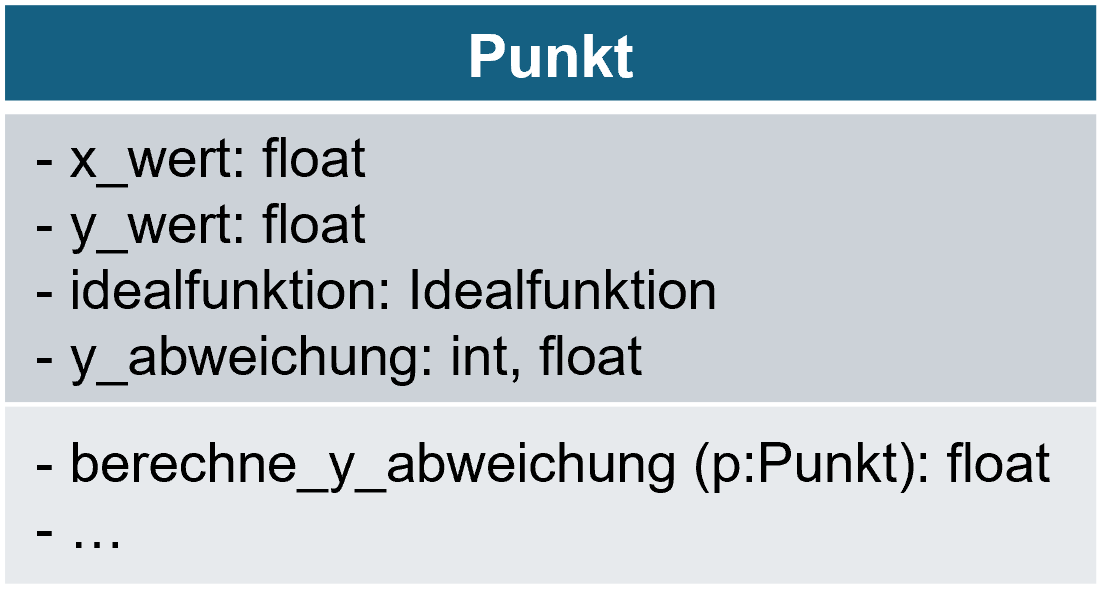
\includegraphics[scale=0.78]{Grafik_Klasse_Punkt}
	\caption{Attribute und Methoden der Klasse Punkt}
	\label{fig:Punkt}
\end{figure}
Die Klasse Punkt ist eine alleinstehende Klasse, die von keiner weiteren Klasse erbt bzw. an eine weitere Klasse vererbt. Die Grundlage der Klasse Punkt ist der X- und Y-Wert. Bei der Erzeugung einer Instanz der Klasse Punkt müssen die beiden Werte zwingend als Attribute übergeben werden. \\
\\
Die Klasse Punkt findet unter anderem Anwendung beim Export der Punkte aus der Klasse Datensatz/Funktion (siehe Methode hole\_punkte(), Kapitel \ref{fig:Datensatz}). Außerdem wird die Methode berechne\_y\_abweichung(p:Punkt) verwendet, um bei der Berechnung für Aufgabenteil 2 die Y-Abweichung zwischen zwei Punkten zu ermitteln. Neben den beiden Attributen x\_wert und y\_wert besitzt die Klasse Punkt zwei weitere Attribute. Zum einen kann dem Punkt mit dem Attribut idealfunktion eine Idealfunktion (Instanz der Klasse Idealfunktion) zugewiesen werden. Zum anderen kann die entsprechende Y-Abweichung zwischen dem Testpunkt und der Idealfunktion unter dem Attribut y\_abweichung hinterlegt werden. 

\section{Exception-Handling}
\label{sec:Exception}
Das Exception-Handling bzw. die Ausnahmebehandlung beschreibt das Bereinigen von Programmfehlern, die auf äußere Umstände zurückzuführen sind. Unter einem Programmfehler (Ausnahme) ist eine Unterbrechung des normalen Programmablaufs zu verstehen. Ohne Behebung des Programmfehlers kann der Programmablauf nicht fortgesetzt werden. Umgesetzt wird das Exception Handling, indem im Fall eines Programmfehlers eine Behandlungsmaßnahme anstelle des eigentlich vorgesehenen Programmcodes ausgeführt wird. Realisiert wird dieses Verfahren in Python durch sogenannte try-except-Blöcke. Der try-Block beinhaltet den Programmcode, der mit dem Exception-Handling behandelt werden soll. Tritt im try-Block eine Ausnahme auf, wird der except-Block ausgeführt. Das Programm wird hierbei nicht beendet, sondern es wird der Programmcode im except-Block ausgeführt.  Python bietet eine Reihe von Standard-Exceptions, die eine qualifizierte Reaktion je nach Ausnahmetyp ermöglichen. \\
Außerdem bietet Python die Möglichkeit, mit der raise-Anweisung benutzerdefinierte Ausnahmeklassen zu aktivieren (Steyer, 2018, S.181-193).\\
In dem vorliegende Python-Programm werden sowohl Standard-Ausnahmen als auch benutzerdefinierte Ausnahmen verwendet. Die implementierten benutzerdefinierte Ausnahmen können Tabelle \ref{tab:ben_Ausnahmen} entnommen werden.
\begin{table}[!h]
\centering
\begin{tabularx}{0.95\textwidth}{|l|X|}
\hline
\textbf{Exception-Klasse} & \textbf{Funktionalität}\\
\hline
DatensatzError() & Abfangen von Ausnahmen in der Klasse Datensatz.\\
\hline
FunktionError() & Abfangen von Ausnahmen in der Klasse Funktion.\\
\hline
PunktError() & Abfangen von Ausnahmen in der Klasse Punkt.\\
\hline
CSVError() & Abfangen von Ausnahmen beim Import einer CSV-Datei.\\
\hline
\end{tabularx}
\caption{Benutzerdefinierte Ausnahmen}
\label{tab:ben_Ausnahmen}
\end{table}

Es ist zu erkennen, dass es für jede Klasse eine eigene Ausnahmebehandlung gibt, die in der Konsole ausgegeben wird. So wird beim Block in die Konsole sofort deutlich, in welcher Klasse eine Ausnahme aufgetreten ist.\\
Da bei der Erzeugung einer Instanz der Klasse Datensatz nicht zwingend ein Pandas-Dataframe übergeben werden muss (siehe Kapitel \ref{fig:Datensatz}), findet das Exception-Handling hier bei jeder Methode Anwendung. Das ist notwendig, da die meisten Methoden der Klasse Datensatz ein Pandas-Dataframe als Grundlage benötigen. Ist jedoch noch kein Pandas-Dataframe hinterlegt, können die Methoden nicht korrekt ausgeführt werden. Es werden die Ausnahmen abgefangen und in der Konsole ausgegeben. Da ein weiterer Ablauf des Programms in diesen Fällen nicht möglich wäre, wird das Programm bei der Ausnahmebehandlung abgebrochen. So kann der Anwender direkt die Fehlerart und die Stelle, an der die Ausnahme auftritt, erkennen.\\
Da bei er Erzeugung einer Instanz der Klasse Funktion zwingend ein Pandas-Dataframe zugewiesen werden muss (siehe Kapitel \ref{sub:Funktion}), ist keine Ausnahmebehandlung bei den Methoden notwendig, die lediglich Daten des Pandas-Dataframe zurückgeben. 
Weitere Ausnahmebehandlung finden Anwendung bei Methoden zur Berechnung der Idealfunktion bzw. der Passung der Testpunkte. Außerdem wird bei jedem Setzen von Variablen über klassenspezifische Methoden geprüft, ob die zugewiesene Variable den korrekten Datentyp besitzt.  \\
Bei der Klasse Punkt (siehe Kapitel \ref{sub:Punkt}) verhält es sich ähnlich wie bei der Klasse Funktion. Auch bei der Erzeugung einer Instanz der Klasse Punkt wird überprüft, ob die zugewiesenen Variablen einen korrekten Datentyp besitzen. \\
Eine Besonderheit bei den benutzerdefinierten Ausnahmebehandlungen ist der CSVError. Ist der als Default hinterlegte Dateipfad oder der vom Nutzer ausgewählte Dateipfad keine CSV-Datei, wird der CSV-Error ausgelöst. Der Anwender erkennt nun in der Python-Konsole, dass es Probleme mit dem Import einer CSV-Datei gibt und kann entsprechend reagieren.\\
Neben den benutzerdefinierten Exception-Handlings werden im vorliegenden Python-Programm auch Standard-Exception-Handlings verwendet. Diese werden immer dann verwendet, wenn Attribute einer Klasse zurückgegeben werden sollen, die zuvor berechnet und zugewiesen werden müssen. Ein Beispiel hierfür ist der AttributeError beim Aufrufen der Methode hole\_idealfunktion() der Klasse Trainingsfunktion (siehe \abbildung{fig:Datensatz}). Das Attribut ideal\_funktion wird erst durch das Aufrufen der Methode suche\_idealfunktion(datensatz) belegt. Wird nun die Methode hole\_idealfunktion() vor der Klasse suche\_idealfunktion(datensatz) aufgerufen, tritt ein Programmfehler auf. Dieser Programmfehler wird mittels des AttributeError abgefangen.

\chapter{Lösungen der Aufgabenstellungen}
\label{cha:Lösung}
In den folgenden Kapiteln werden die Lösungen der Aufgabenstellungen präsentiert. Außerdem werden die Visualisierungen der Lösungen dargestellt und erklärt. 

\section{Passungen aus Trainings- und Idealfunktion}
Das Ziel der Aufgabenstellung 1 ist es, den vier gegebenen Trainingsfunktion jeweils eine Idealfunktion zuzuweisen (siehe Kapitel \ref{sec:Aufgabenteil1}). Folgende Tabelle zeigt die Passungen aus Trainings- und Idealfunktion. 

\begin{table}[!h]
\centering
\begin{tabularx}{0.5\textwidth}{|l|X|}
\hline
\textbf{Trainingsfunktion} & \textbf{Idealfunktion}\\
\hline
Y1 & Y36\\
\hline
Y2 & Y11\\
\hline
Y3 & Y2\\
\hline
Y4 & Y33\\
\hline
\end{tabularx}
\caption{Passungen aus Trainings- und Idealfunktion}
\label{tab:Passungen}
\end{table}
Die Visualisierung der Ergebnisse erfolgt durch das Abbilden der Trainings- sowie Idealfunktion untereinander. Zusätzlich zeigt die dritte Grafik die Y-Abweichungen zwischen Trainings- und Idealfunktion. \abbildung{fig:Train1} zeigt exemplarisch die Visualisierung für die Trainingsfunktion Y1.
\begin{figure}[!h]
	\centering
	\includegraphics[scale=0.32]			  {Trainingsfunktiony1_Lösung}
	\caption{Visualisierung der Trainingsfunktion 1}
	\label{fig:Train1}
\end{figure}
\\
Es ist deutlich zu sehen, dass die Trainingsfunktion keine geradlinige Funktion ist. Sie besteht aus einer Vielzahl von Messungen, die von einer Idealfunktion leicht abweichen. Die Idealfunktion ist in der mittleren Grafik (siehe \abbildung{fig:Train1}) dargstellt. Die Abweichungen der Trainingsfunktion von der Idealfunktion sind in der untersten Grafik dargstellt. Zu sehen ist, dass keine Abweichung größer als 0.5 bzw. kleiner als -0.5 ist.\\
Das Python-Programm erzeugt für jede Trainingsfunktion eine ähnliche Grafik, die im selben Ordner gespeichert wird, in dem sich die Python-Datei befindet. 

\section{Anpassbare Testpunkte}
Die Aufgabenstellung 2 fordert das Zuweisen von den gegebenen Testpunkte zu einer oder mehreren Idealfunktionen. Hierfür ist ein Testkriterium vorgegeben, das die Testpunkte erfüllen müssen (siehe \ref{sec:Aufgabenteil2}. Jeder Idealfunktion kann mindestens ein Testpunkt zugewiesen werden. Tabelle \ref{tab:Testpunkte} zeigt die Anzahl der Testpunkte je Idealfunktion. 

\begin{table}[!h]
\centering
\begin{tabularx}{0.5\textwidth}{|l|X|}
\hline
\textbf{Idealfunktion} & \textbf{Anzahl Testpunkte}\\
\hline
Y2 & 9\\
\hline
Y11 & 11\\
\hline
Y33 & 11\\
\hline
Y36 & 4\\
\hline
\end{tabularx}
\caption{Anzal Testpunkte pro Idealfunktion}
\label{tab:Testpunkte}
\end{table}

Die Visualisierung der Ergebnisse erfolgt durch das Darstellen der Idealfunktion als Graphen. In dieselbe Grafik sind die passenden Testpunkte als Punkte dargestellt, sodass ihre Abweichungen von der Idealfunktion grob abgegriffen werden können.

\begin{figure}[!h]
	\centering
	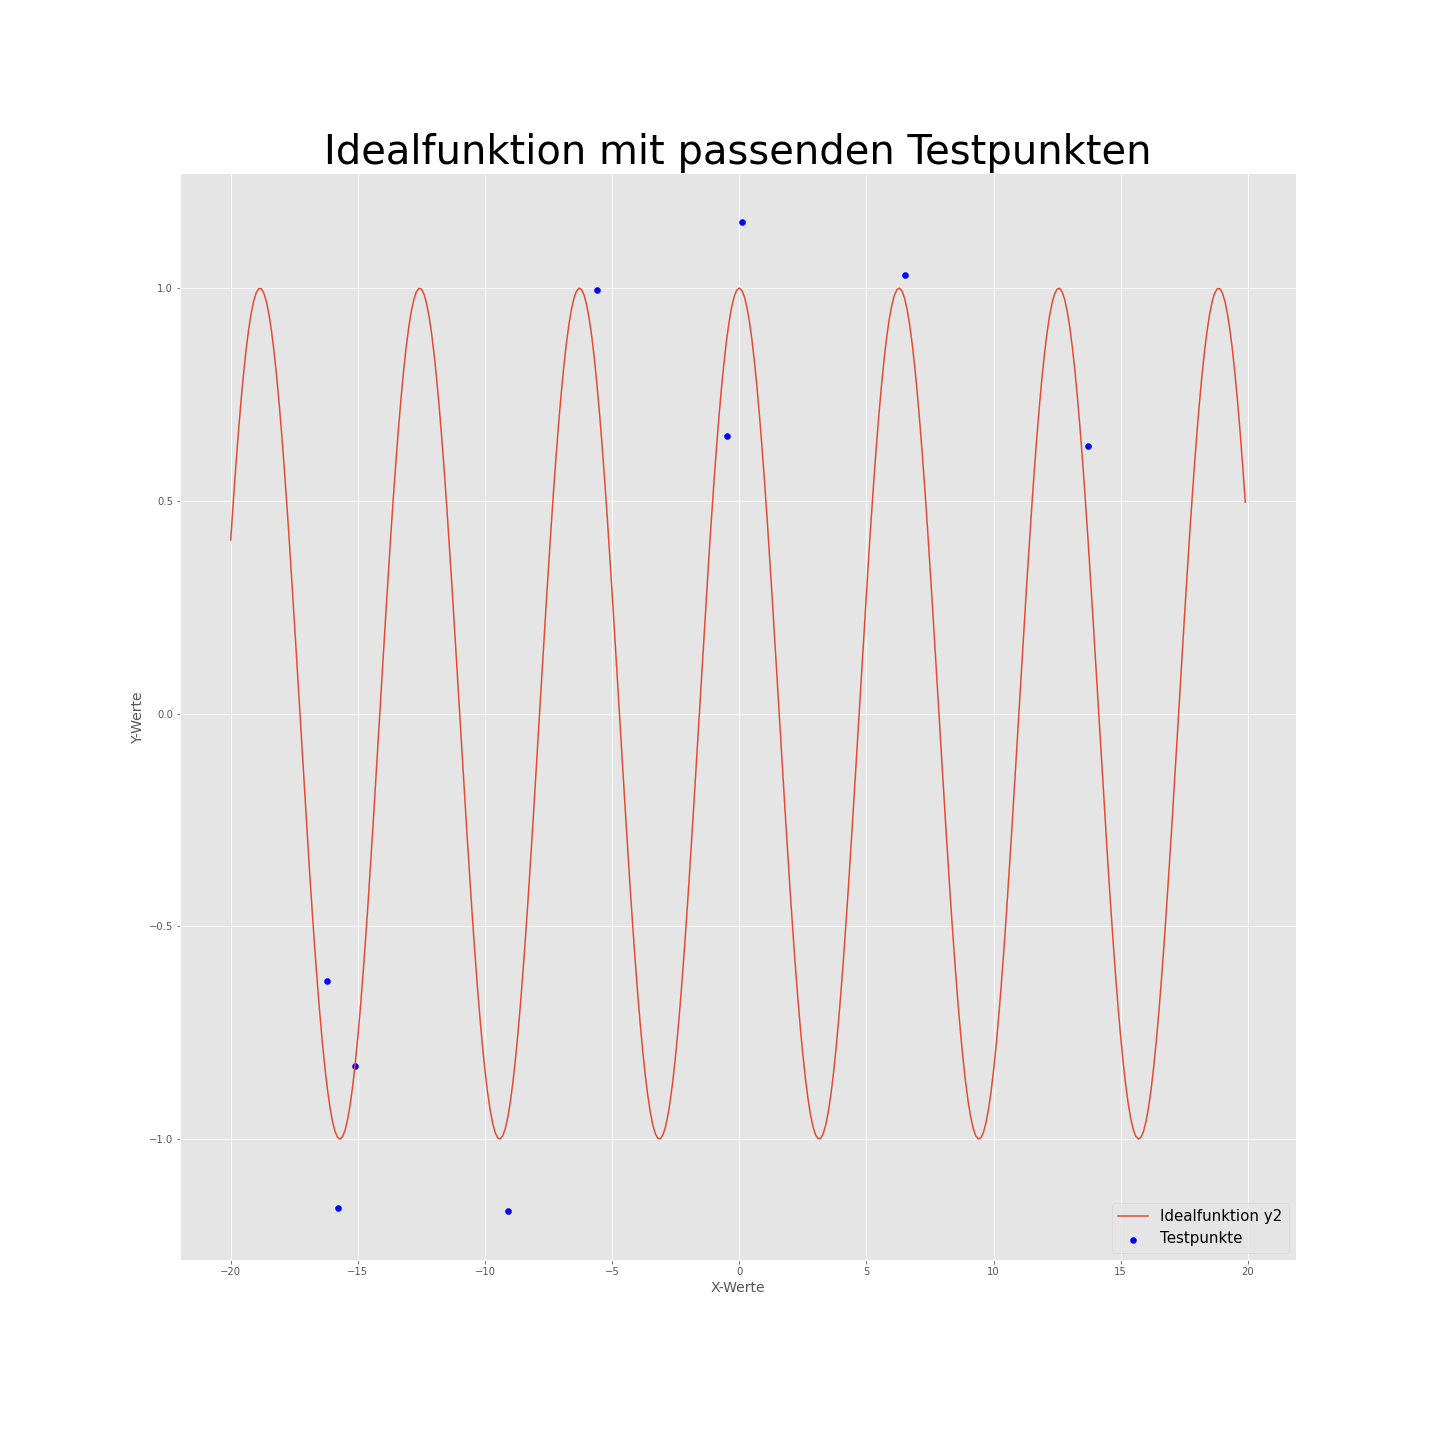
\includegraphics[scale=0.25]			  {Idealfuntionfunktion_y2_Testpunkte}
	\caption{Visualisierung der Idealfunktion Y2 und Testpunkte}
	\label{fig:Ideal2}
\end{figure}

\abbildung{fig:Ideal2} zeigt die Visualisierung der Aufgabenstellung 2 exemplarisch für die Idealfunktion Y2. Die Abweichungen zwischen den Testpunkten und der Idealfunktion werden abgespeichert und später in eine entsprechende SQLite-Datei exportiert (siehe Kapitel \ref{sec:sqlite}). Für jede der vier Idealfunktionen wird eine nach demselben Muster erstellte Grafik (siehe \abbildung{fig:Ideal2}) erzeugt und gespeichert. 

\section{SQLite-Export}
\label{sec:sqlite}
Laut Aufgabenstellung sollen der Trainingsdatensatz, der Idealdatensatz und die Ergebnisse aus Aufgabenstellung 2 jeweils in eine SQLite-Datenbank (Datei) exportiert werden. Der Zugriff auf die SQLite-Datenbank erfolgt wie in Kapitel \ref{sec:SQL} beschrieben  mit Hilfe der SQL-Alchemy-Bibliothek. Das vorliegende Python-Programm erzeugt hierfür drei separate SQLite-Dateien, die jeweils nur eine Tabelle enthalten. \\
Der Trainings- und Idealdatensatz muss nicht weiter verändert werden und kann dementsprechend ohne weitere Bearbeitung exportiert werden. Die Ergebnisse der Aufgabenstellung 2 werden zum einfacheren Export in einer Instanz der Klasse Datensatz (siehe Kapitel \ref{fig:Datensatz}) gespeichert. Somit liegen die Ergebnisse als Pandas-Dataframe vor und können exportiert werden. \abbildung{fig:DBTestpunkte} zeigt die Struktur der Tabelle der resultierenden SQLite-Datenbank. 
\begin{figure}[!h]
	\centering
	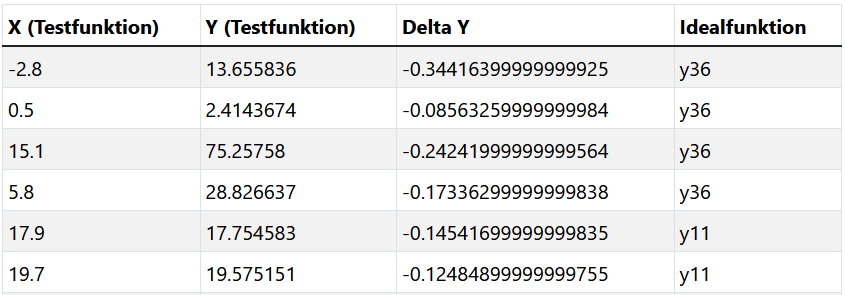
\includegraphics[scale=0.9]{Datenbank_2}
	\caption{Struktur der SQLite-Datenbank für die Testpunkte}
	\label{fig:DBTestpunkte}
\end{figure}
\section{Anwendung von Unit-Tests}
Wie in \ref{sec:UnitTest} beschrieben wird die Funktionalität des vorliegenden Programms mittels Unit-Tests überprüft. Es werden im Wesentlichen drei unterschiedliche Funktionalitäten der konstruierten Klassen getestet. \\
Zum einen wird die jeweilige Konstruktor-Methode je Klasse überprüft. Mit Hilfe der Konstruktormethode (\_\_init\_\_) können  einer Instanz einer Klasse ein oder mehrere Anfangswerte zugewiesen werden (Theis, 2017, S.206). Im Unit-Test-Modul werden Instanzen der drei Klassen (siehe Kapitel \ref{sec:OOP}) bewusst falsche Anfangswerte übertragen. Es wird nun geprüft, ob die richtigen Fehlermeldungen ausgegeben werden. In diesem Fall handelt es sich um die benutzerdefinierten Ausnahmen. \\
Außerdem werden die Getter- und Setter-Methoden der Klassen geprüft. Hier wird geprüft, ob die Klassen die korrekten Werte der privaten bzw. geschützten Attribute zurückgeben. \\
Zuletzt werden die Methoden der Klassen überprüft, die Berechnungen durchführen. Mit einfachen Datenstrukturen werden die Rechenmethoden durchgeführt und geprüft, ob die Methoden das richtige Ergebnis zurückgeben. 

\chapter{Reflexion des Python-Programms}
\label{cha:Reflexion}
In diesem Kapitel wird das vorliegende Python-Programm, welches die Grundlage dieser Hausarbeit bildet, reflektiert. Es wird die verwendete Struktur erklärt und mögliche Alternativen dargelegt und erörtert. \\
Die am kritischsten zu hinterfragende Klasse im Programm-Code ist die Klasse Datensatz. Beim Erzeugen einer Instanz der Klasse Datensatz muss nicht zwingend eine Anfangswert übertragen werden (siehe \abbildung{fig:Datensatz}). Das führt dazu, dass das Konstruieren sowie Anwender der weiteren Methode komplizierter ist, als wenn zwingend ein Pandas-Dataframe zugewiesen werden müsste. Bei jeder Anwendung einer Methode muss überprüft werden, ob dem Objekt ein Pandas-Dataframe zugewiesen wurde. Das führt dazu, dass die Anwendung der Klasse Datensatz fehleranfällig wird. Mit Hilfe des Exception-Handlings (siehe Kapitel \ref{sec:Exception}) werden die zu erwartenden Ausnahmen jedoch gezielt abgefangen. Der Anwender bekommt in der Python-Konsole eine Fehlermitteilung und kann entsprechend reagieren.\
Der Vorteil eines Konstruktors ohne zwingende Zuweisung eines Attributs ist in diesem Fall, dass die Instanz der Klasse Datensatz mit einer Methode durch eine CSV-Datei gefüllt werden kann. Es wird dem Anwender eine Möglichkeit geboten, den Pfad einer CSV-Datei zu übertragen, wobei anschließend aus den Daten der CSV-Datei ein Pandas-Dataframe erzeugt wird.\\
Weiterhin kann kritisiert werden, dass die Klasse Datensatz zum Großteil lediglich Methoden der Klasse Pandas-Dataframe beinhaltet. So kann der Eindruck entstehen, dass Klasse Datensatz überflüssig ist. Alle Funktionen/Methoden könnten im normalen Programm-Code über die Funktionen eines Pandas-Dataframes ausgeführt werden. Die Klasse Datensatz hat jedoch in erster Linie den Auftrag, dem Anwender die Bearbeitung der Aufgabenstellung zu erleichtern. Sie ist eine aufgabenspezifische Klasse, welche die benötigten Funktionen des komplexen Pandas-Dataframes bündelt. Der Anwender muss sich nicht mit den Funktionen eines Pandas-Dataframes auseinandersetzen, sondern hat alle Methoden, die für die Lösung der Aufgabe notwendig sind, einfach formuliert vorliegen. Ein Beispiel hierfür ist die Methode anzahl\_zeilen(). Dem Anwender ist sofort klar, welchen Wert diese Methode zurückgibt. Die entsprechende Funktion bzw. das Attribut des Pandas-Dataframes (dataframe.shape[0]) hingegen macht nicht deutlich, was zurückgegeben wird. \\
Außerdem wäre es möglich, auf die Klasse Funktion zu verzichten. Da ihre Grundlage ebenfalls ein Pandas-Dataframe ist, ähnelt sie sehr stark der Klasse Datensatz. Sie besitzen ähnliche Methoden und Attribute. Der entscheidende Unterschied ist jedoch, dass die Klasse Funktion nur die ersten zwei Spalten des Pandas-Dataframes verarbeitet. Somit werden bei der Klasse Funktion nur die Spalte mit den X-Werten und die Spalte mit den ersten Y-Werten berücksichtigt. Für die Klasse Funktion ergibt es nur Sinn, ein zweispaltiges Pandas-Dataframe als Anfangsattribut zu übertragen. Durch die Vererbungshierarchie können Methoden aus der Klasse Datensatz, die für beide Klassen notwendig sind, auch von der Klasse Funktion verwendet werden. Außerdem besitzen die beiden genannten Klassen einen weiteren Unterschied, der eine Trennung der Klassen durch Vererbung sinnvoll macht. Die Klasse Datensatz dient vielmehr zur Speicherung und Verarbeitung der Eingangs- und Ausgangsdaten. Die Klasse Funktion hingegen führt die elementaren Berechnungen und Vergleiche durch und bestimmt somit die Ergebnisse der Aufgabenstellungen. \\
Ein weitere Möglichkeit, den Programm-Code zu verkürzen, besteht durch das Verwenden von ausschließlich einer Klasse Funktion. Die Methoden und Attribute der abgeleiteten Klassen Trainings- und Idealfunktion könnten auch in der Klasse Funktion implementiert werden. Da die beiden abgeleiteten Klassen jedoch jeweils eine Methode besitzen, die für die Lösung der Aufgabenstellung wichtig ist, ist hier eine strikte Unterscheidung sinnvoll. Es wird eine Trennung zwischen den beiden Funktionstypen geschaffen, da bspw. die Idealfunktion deutlich mehr Attribute als die Trainingsfunktion benötigt. Außerdem ist bei der Erzeugung einer Instanz der Klassen erkennbar, um welche Art von Funktion es sich handelt. Die Unterscheidung zwischen Trainings- und Idealfunktion kann bei nur einer Klasse Funktion alternativ durch die Bezeichnung/Variable der Instanz der Klasse Funktion verdeutlicht werden. In dem vorliegen Python-Programm ist jedoch die Übersicht bereits durch das Implementieren der beiden Klassen Trainings- und Idealfunktion gegeben. \\
Um den Gedankengang einer objektorientierten Programmierung strikter zu verfolgen, wäre es möglich gewesen, den Programm-Code, der sich außerhalb des Definitionsbereich der Klassen befindet, in die entsprechenden Klassen als Methode zu integrieren. Bei dem genannten Programm-Code handelt es sich um das Erzeugen der Grafiken und der Export der Daten in eine SQLite-Datei. Da die SQL-Alchemy- und Matplotlib-Bibliothek viele Parameter zur Einstellung der Visualisierung bzw. den Daten-Export besitzen, sind in dem vorliegenden Python-Programm keine entsprechenden Methoden vorzufinden. Es müssten der Methode zu viele Parameter zugewiesen werden, sodass die Übersichtlichkeit verloren geht. Einfacher ist es hier, die Parameter genau an der Stelle im Programm anzugeben, an denen auch die Erzeugung der Grafiken bzw. das Exportieren der Daten vollzogen wird. \\
Der Aufbau der Visualisierungen der Lösung aus Aufgabenteil 1 (siehe \abbildung{fig:Train1}) folgt dem Gedanken der Übersichtlichkeit in dieser Hausarbeit. Alternativ könnten alle Grafiken (Trainingsfunktion, Idealfunktion, Y-Abweichungen) in einer Grafik/Darstellung vereint werden. Der entscheidende Nachteil ist dann, dass der Unterschied zwischen Trainings- und Idealfunktion kaum erkennbar ist. In den vorliegenden Visualisierungen ist deutlich zu erkennen, dass die Trainingsfunktion eine Reihe von Messwerten und die Idealfunktion eine geradlinige Funktion darstellt. Die dargestellten Y-Abweichungen besitzen entlang der Y-Achse einen anderen Maßstab als die Trainings- sowie Idealfunktion. So können die Abweichungen deutlicher dargestellt werden und Ausreißer schnell ausfindig gemacht werden. 


\end{document}